\documentclass{article}
\usepackage[margin=2cm]{geometry}
\usepackage{graphicx}
\usepackage[pages=some]{background}
\usepackage{titling}
\usepackage{tabularx}
\usepackage{tikz}
\usepackage{multicol}
\usepackage{caption}
\usepackage{booktabs}
\usepackage{hyperref}
\usepackage{float}
\usepackage{adjustbox}
\usepackage{tabularx}
\usepackage{amssymb}
\usepackage{amsmath}

\geometry{a4paper}

\backgroundsetup{
    scale=1,
    angle=0,
    opacity=1,
    contents={%
        
\includegraphics[width=\paperwidth,height=\paperheight]{institution_logo.jpg}
    }
}

\newcommand{\subtitle}[1]{
    \posttitle{
        \par\end{center}
        \begin{center}\large#1\end{center}
        \vskip0.5em}
}

\title{ME-415}
\subtitle{REFRIGERATION AND BUILDING MECHANICAL SYSTEMS}
\author{TOPIC : COOLING LOAD ESTIMATION}

\begin{document}
\begin{titlepage}
    \centering
    
    {\Huge\bfseries\maketitle}
    \vspace{1cm}
    
\includegraphics[width=8cm]{institution_logo.jpg}
    \vspace*{3cm}
    \begin{multicols}{2}
      \begin{quote}
        
        \begin{flushleft}
          
          \hspace{1cm} Submitted by - \\
          \hspace{1cm} Name : \textbf{Md. Hasibul Islam}\\
          \hspace{1cm} Roll : 1810009\\
          \hspace{1cm} Dept. : Mechanical Engineering\\ 
          \hspace{1cm} Section : A \\
          \hspace{1cm} Submitted to - \\
          \hspace{1cm} \textbf{Dr. Arif Hasan Mamun} \\ 
          \hspace{1cm} Professor, Mechanical Engineering \\ 
          \hspace{1cm} Bangladesh University of \\ \hspace{1cm} Engineering \& Technology (BUET)
        \end{flushleft}
      \end{quote}
      \end{multicols}
    \vfill
\end{titlepage}

\tableofcontents
\pagebreak

\section{CAD model of Room}

\begin{figure}[H]
    \centering
    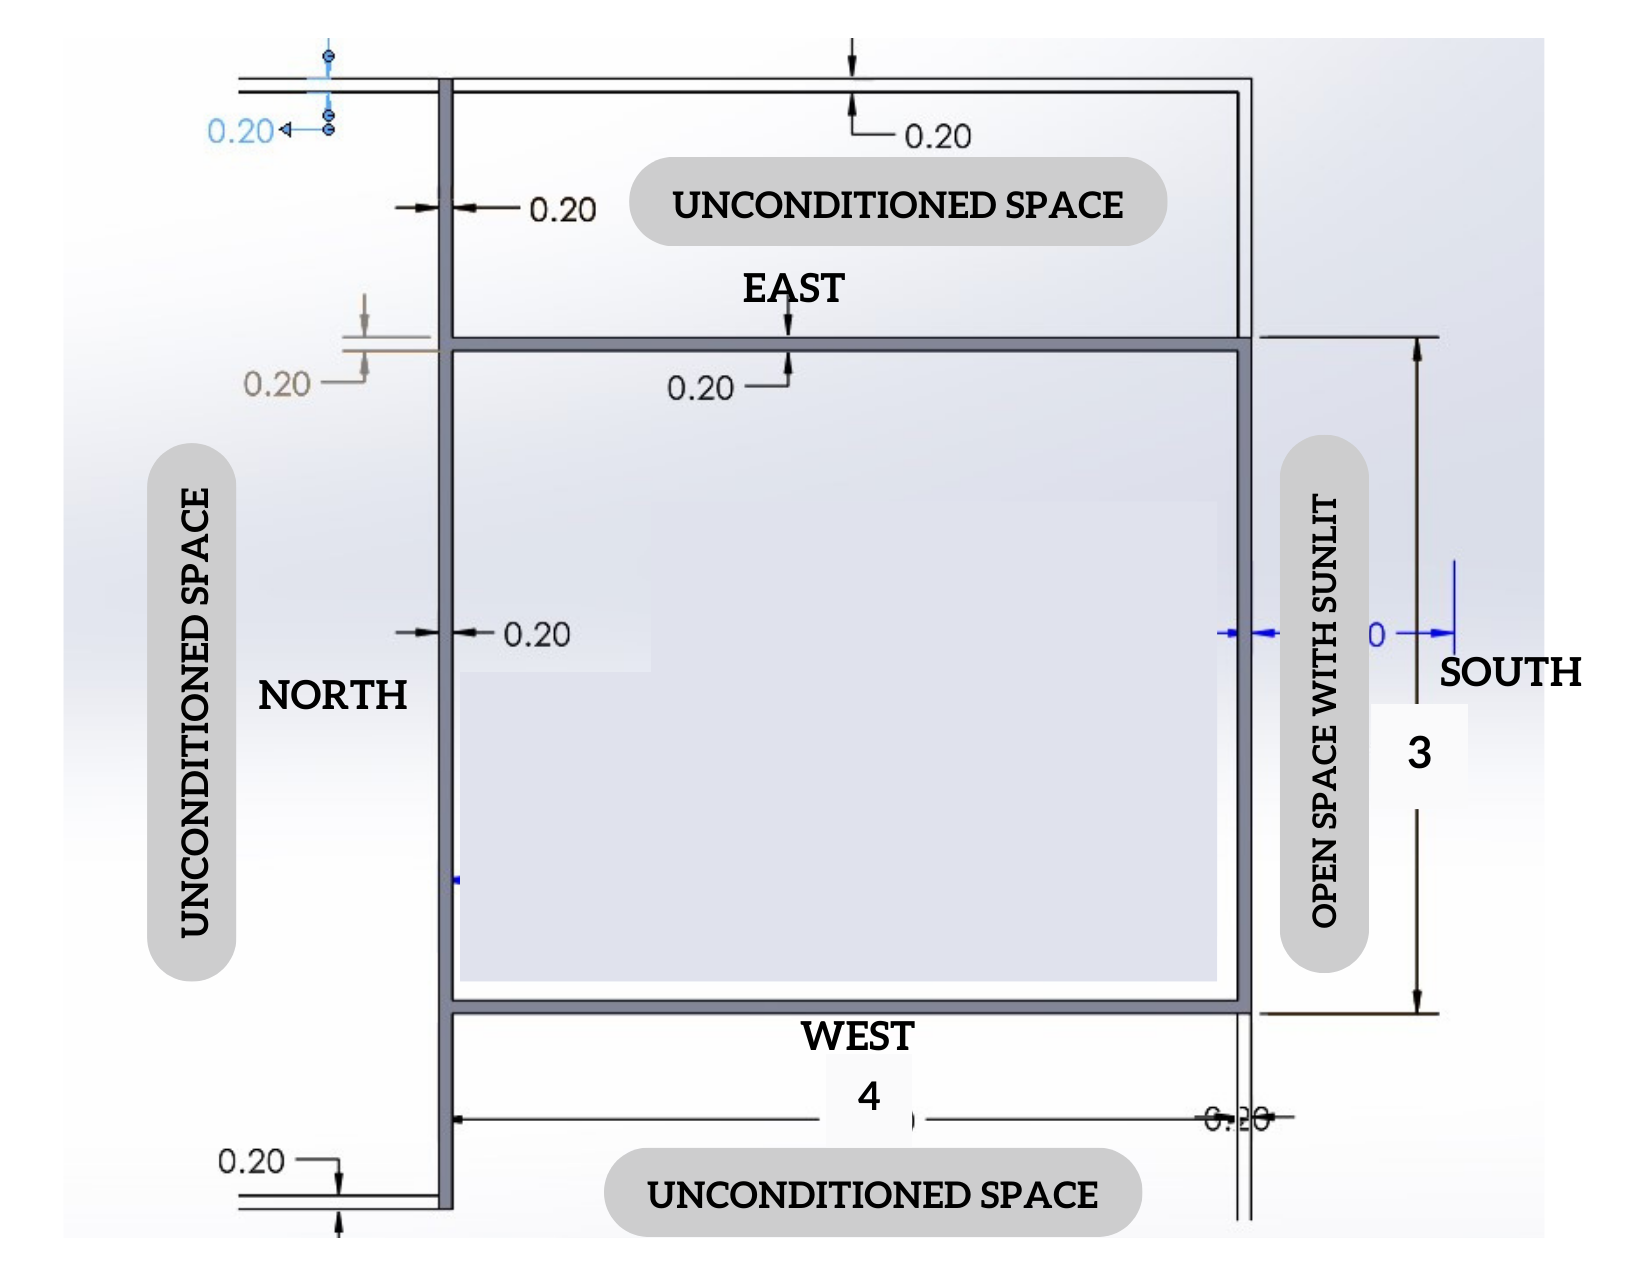
\includegraphics[width=0.99\textwidth]{img/img1.png}
    \caption{Top View of Room}
    \label{fig:1}
\end{figure}

\begin{figure}[H]
    \centering
    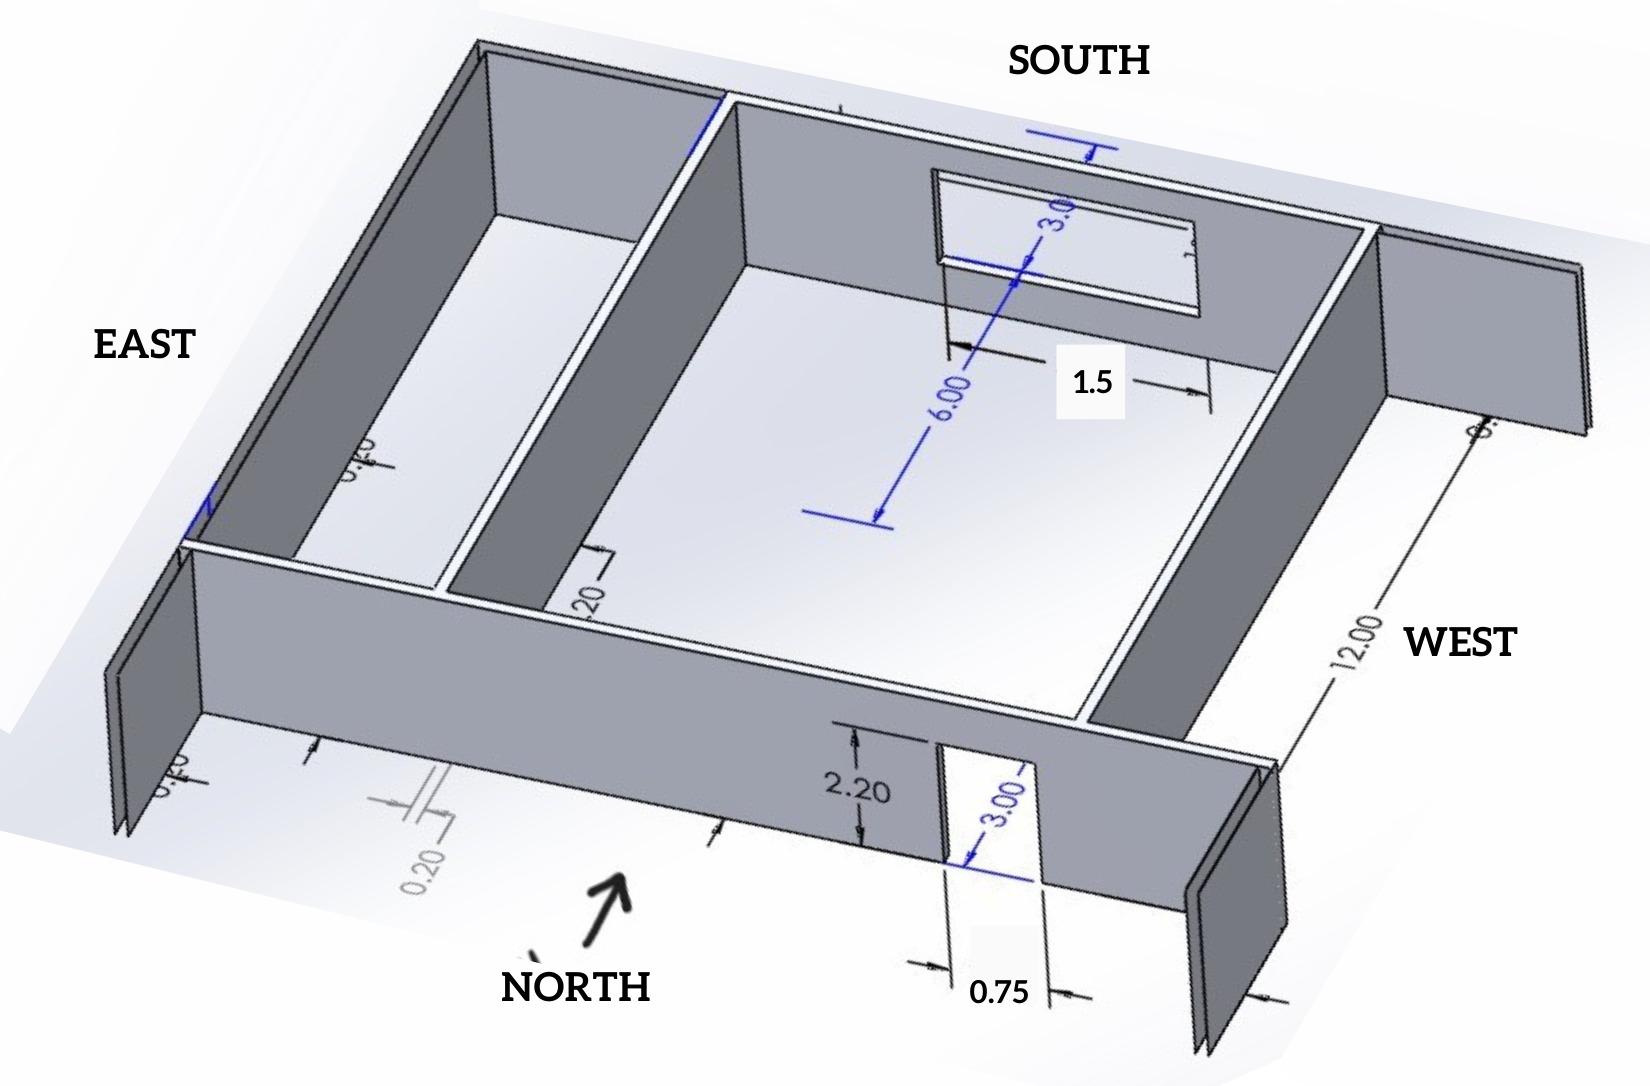
\includegraphics[width=0.99\textwidth]{img/img2.png}
    \caption{North to south view of Room}
    \label{fig:2}
\end{figure}
\vspace{1cm}
\begin{figure}[H]
    \centering
    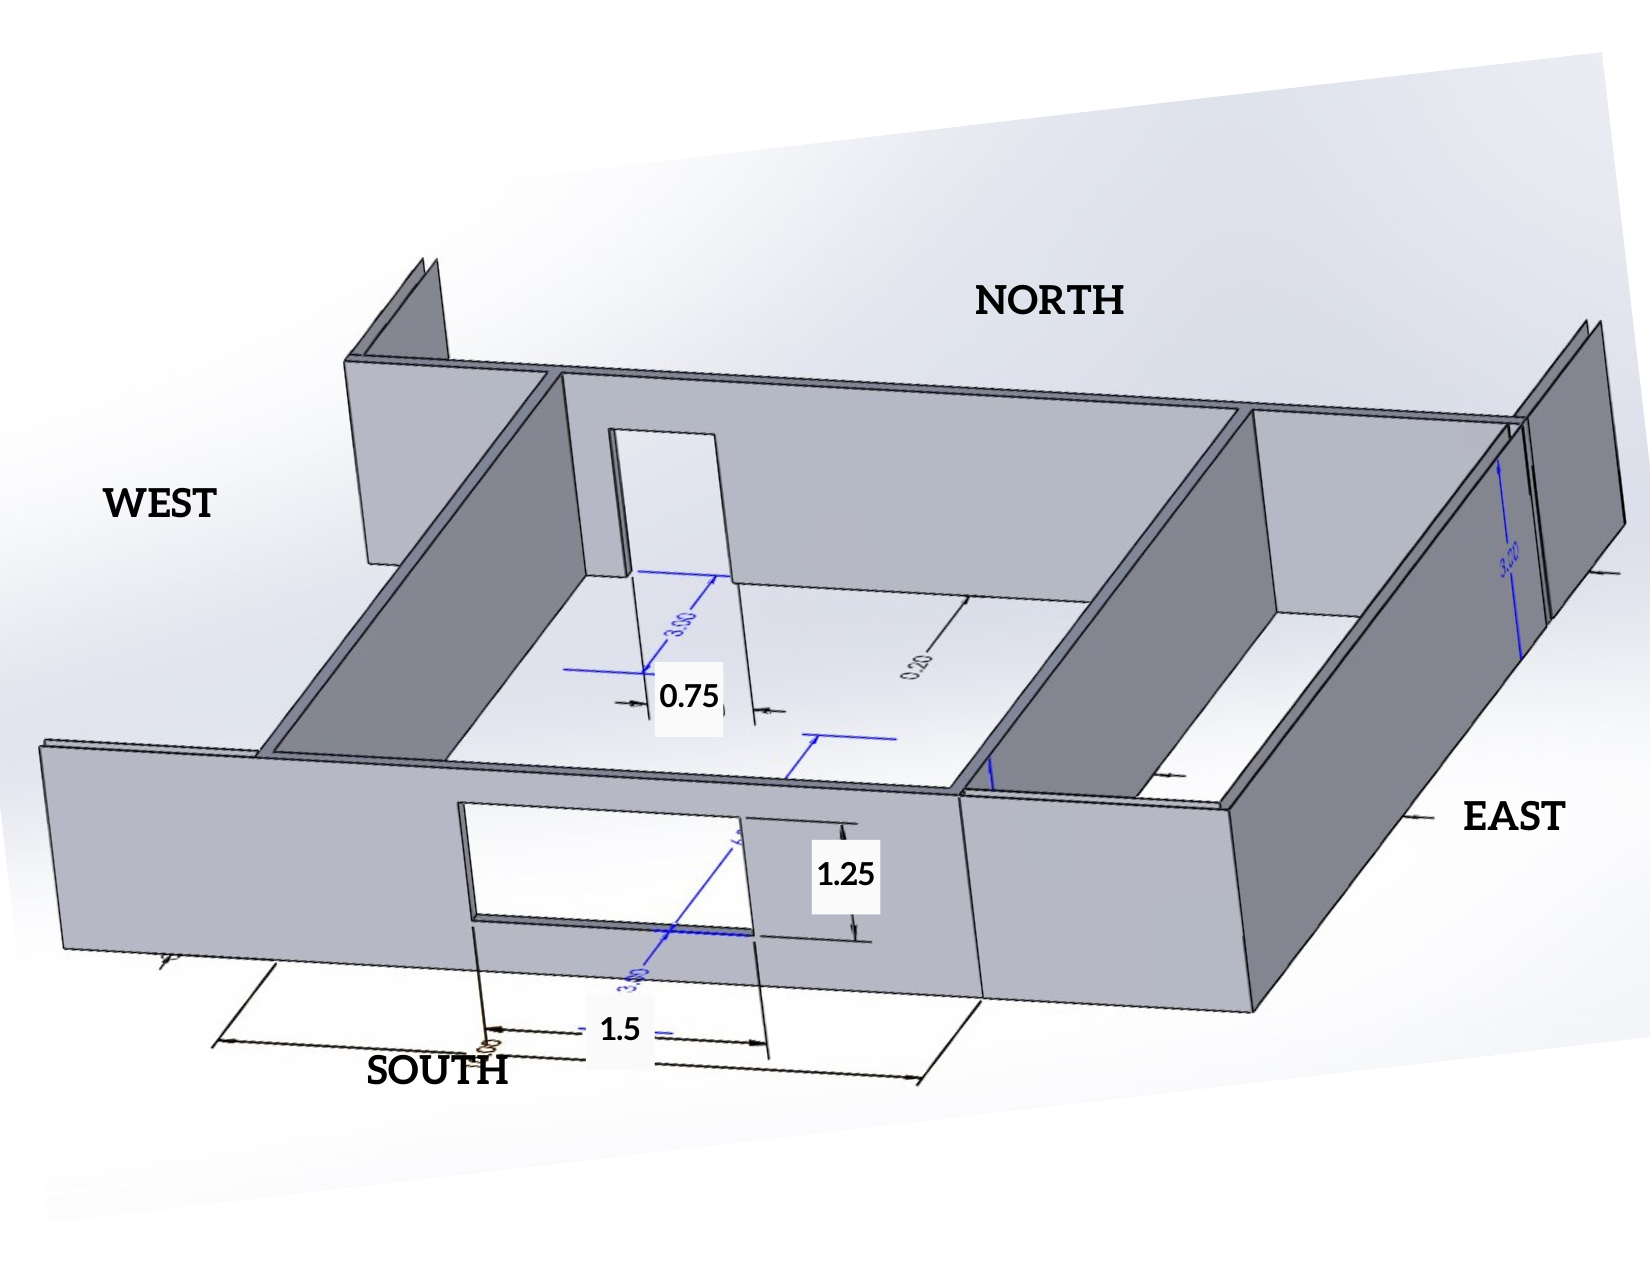
\includegraphics[width=0.99\columnwidth]{img/img3.png}
    \caption{South to North view of Room}
    \label{fig:3}
\end{figure}
\pagebreak

\section{Model Specification}
\begin{enumerate}
  \item \textbf{Date \& Time:} April Month, at 5 pm 
  \item \textbf{Location:} Lakshmipur, Bangladesh
  \item \textbf{Temperature:} 25.5 $^{\circ}$C
  \item \textbf{Relative Humidity:} 50\%
  \item \textbf{Dimensions:}
  \begin{itemize}
    \item Length : 12 m
    \item Width : 10 m
    \item Height : 3 m
    \item Window : 4 m $\times$ 1.75 m (on south wall)
    \item Door : 2.2 m $\times$ 1.50 m (on north wall)
  \end{itemize}
  \item \textbf{Surroundings}:
  \begin{itemize}
    \item South side : Open Space \& sunlit presence
    \item East side : Unconditioned Space 
    \item North side : Unconditioned Space 
    \item West side : Unconditioned Space 
  \end{itemize}
  \item \textbf{Construction:}
  \begin{itemize}
    \item \textbf{Roof} : Type-4 with 50 mm insulation without suspended ceiling. 
    \item \textbf{All walls (N, E, S, W)} : 150 mm  brick with 25 mm plaster on both sides.
    \item \textbf{Door} : 25 mm thick hard wooden door.
    \item \textbf{Window} : U = 2.5 $W/m^2-K$ with 15 mm thick glass of light construction.
    \item \textbf{Floor} : No heat transfer through floor. 
  \end{itemize}
  \item \textbf{Other factors:}
  \begin{itemize}
    \item 2 occupants seated with 1 using Laptop 
    \item 1 light of 25 W with flouroscence light 
    \item No other electronic devices 
    \item Lights and occupants from 11 am to 10 pm 
    \item Air change rate = 1.0 $/hr$
  \end{itemize} 
\end{enumerate}
\pagebreak

\section[Heat Conduction through Partition walls / glasses]{Heat Conduction through Partition walls / glasses}
\subsection{Roof}
\begin{center}
  \textbf{Type-4 with 50 mm insulation without suspended ceiling} \\
  
  From Table-12(a),
  Layers : \textbf{A0 E2 E3 B6 C12 E0} \\ 
\end{center}

Now, reading the values from table-16,

\begin{table}[ht]
  \centering
  \begin{adjustbox}{width=\textwidth}
  \begin{tabularx}{\linewidth}{p{0.15\linewidth} p{0.6\linewidth} p{0.18\linewidth}}
      \hline
      Layers & Layers Details & Resistance \\
      \hline
      A0 & Outside Surface Resistance & 0.059 \\
      E2 & 12 mm slag or stone & 0.099 \\
      E3 & 10 mm felt and membrane & 0.050 \\
      B6 & 50 mm insulation & 1.173 \\
      C12 & 50 mm heavy weight concrete & 0.029 \\
      E0 & Inside surface resistance & 0.121 \\
      \hline
  \end{tabularx}
  \end{adjustbox}
  \caption{Roof Layers}
  \label{tab:Roof}
  \end{table}
  Total resistance, R = 1.581 \\
  \hspace*{0.3cm} $\therefore$ U = 1/R = 0.653 \\

  \vspace{0.5cm}

  \subsection{Walls}
  \begin{center}
    \textbf{North, East, South \& West Walls: \\150 mm brick with 25 mm plaster on both sides} \\
  \end{center}
  From table 16,
  \begin{itemize}
    \item For C4 : 100 mm common brick, k = 0.727 $W/m-K$\\
    Now, resistance for 150 mm brick,\\ $R_2$ = 0.150/0.727 = 0.206 
    \item For E1 : 20 mm plaster, k = 0.7277 $W/m-K$\\
    Now, resistance for 25 mm plaster,\\ $R_1 = R_3$ = 0.025/0.7277 = 0.0344 
    \item Total resistance, R = $R_o + R_1 + R_2 + R_3 + R_i$ \\= 0.059 + 0.0344 + 0.206  + 0.0344 + 0.121 \\= 0.4548 
    \item U = 1/R = 2.199 $W/m^2-K$ 
  \end{itemize}

  \vspace{0.5cm}
  \subsection{Window}
  \begin{center}
    \textbf{15 mm thick glass of light construction} \\
  \end{center}

  \begin{itemize}
    \item U = 2.5 $W/m^2-K$
  \end{itemize}

  \vspace{0.5cm}
  \subsection{Door}
  \begin{center}
    \textbf{25 mm thick hard wooden door} \\
  \end{center}

  \begin{itemize}
    \item Door size : 2.2 m $\times$ 1.5 m 
    \item From table-17.6, Hard wood : Oak, k = 0.16 $W/m-K$\\
    Now, resistance for 25 mm thick door,\\ $R_{door}$ = 0.025/0.16 = 0.156 
    \item Total resistance, R = $R_o + R_{door} + R_i$ \\= 0.059 + 0.156 + 0.121 \\= 0.336 
    \item U = 1/R = 2.976 $W/m^2-K$ 
  \end{itemize}

  \vspace{0.5cm}
  \subsection{Calculation Table}

  \begin{itemize}
    \item Assuming, $T_o$ = 30.5 $^{\circ}C$ and $T_i$ = 25.5 $^{\circ}C$. 
    \item $T_{o,max} = 33^{\circ}$ for Bangladesh [From table : 9]
  \end{itemize}
  \begin{table}[ht]
    \centering
    \begin{adjustbox}{width=\textwidth}
    \begin{tabularx}{\linewidth}{p{0.10\linewidth} p{0.13\linewidth} p{0.13\linewidth} p{0.13\linewidth} p{0.13\linewidth} p{0.13\linewidth} p{0.13\linewidth}}
        \hline
        SI. no. & Item & Description & A & U & TD & Q (watt) \\
        \hline
        1 & Partition wall & North & 26.7 & 2.199 & 5.0 & 293.57 \\
        2 & Partition wall & East & 36 & 2.199 & 5.0 & 395.82 \\
        3 & Partition wall & West & 36 & 2.199 & 5.0 & 395.82 \\
        4 & Partition wall & South & 23 & 2.199 & 7.5 & 379.33 \\
        5 & Partition glass & South & 7 & 2.50 & 7.5 & 131.25 \\
        6 & Door & North & 3.3 & 2.976 & 5.0 & 49.104 \\
        \hline
        &&&&&& 1644.894 \\
        \hline
    \end{tabularx}
    \end{adjustbox}
    \caption{Heat conduction through partition walls / glasses}
    \label{tab:heat conduction through partition walls / glasses}
    \end{table}
    \vspace*{1cm}

    \section[Heat Conduction through roof \& sunlit walls / glasses]{Heat Conduction through roof \& sunlit walls / glasses}
    \subsection{Roof}
    Parameters:
    \begin{multicols}{2}
      $T_i$ = 25.5 $^{\circ}C$ \\
      $T_{o,max}$ = 33 $^{\circ}C$ \\
      $T_{o,av}$ = 33 - 11/2 = 27.5 $^{\circ}C$ [Table : 9] \\
      CLTD = 37  [Table: 12(b)]\\
      \\
      Correction for Latitude \& month,LM=0 [Table : 13] \\
      Attic Fan Factor, f = 1 \\
      Color adjustment factor, K = 1 [dark color] \\
    \end{multicols}

    \begin{align*}
      CLTD_c &= \left[(CLTD + LM)K + (25.5 - T_i) + (T_{o,av} - 29.4)\right] f \\
      &= \left[(37 + 0)1 + (25.5 - 25.5) + (27.5 - 29.4)\right] 1 \\
      &= 35.1 
    \end{align*}

    \subsection{South Wall}
    Parameters:
    \begin{multicols}{2}
      $T_i$ = 25.5 $^{\circ}C$ \\
      $T_{o,max}$ = 33 $^{\circ}C$ \\
      $T_{o,av}$ = 33 - 11/2 = 27.5 $^{\circ}C$ [Table : 9] \\
      CLTD = 17  [Table: 15]\\
      \\
      Correction for Latitude \& month,LM= -1.6 [Table:13] \\
      Attic Fan Factor, f = 1 \\
      Color adjustment factor, K = 1 [dark color] \\
    \end{multicols}

    \begin{align*}
      CLTD_c &= \left[(CLTD + LM)K + (25.5 - T_i) + (T_{o,av} - 29.4)\right] f \\
      &= \left[(17 - 1.6)1 + (25.5 - 25.5) + (27.5 - 29.4)\right] 1 \\
      &= 13.5
    \end{align*}

    \subsection{Glass}
    From Table-20: \\
    At 5 pm, CLTD = 7  [No correction needed]\\

    \subsection{Calculation Table}
    \begin{table}[ht]
      \centering
      \begin{tabularx}{\linewidth}{p{0.10\linewidth} p{0.13\linewidth} p{0.13\linewidth} p{0.13\linewidth} p{0.13\linewidth} p{0.13\linewidth} p{0.13\linewidth}}
          \hline
          SI. no. & Item & Description & A & U & TD & Q (watt) \\
          \hline
          1 & Roof & Type 4 & 120 & 0.653 & 35.1 & 2750.44 \\
          2 & South wall & Type C4 & 23 & 2.199 & 13.5 & 682.79 \\
          3 & Sunlit glass & South & 7 & 2.50 & 7.0 & 122.5 \\
          \hline
          &&&&&& 3555.73 \\
          \hline
      \end{tabularx}
      \caption{Heat Conduction through Roof and Sunlit Walls/Glasses}
      \label{tab:Heat-Conduction-Roof-Sunlit-Walls-Glasses}
    \end{table}
    \vspace*{1cm}

    \section{Heat Gain}
    \subsection{Solar Heat gain through glass}
    Shading factor, $SF$ = 0.85 [Table : 21, for 15 mm thickness clear glass] \\
    $SHGF_{max}$ = 237 [Table : 18(a), for south wall in April month] \\
    $CLF$ = 0.59 [Table : 19, for south wall at 5 pm] \\ 
    Window area = 4 m $\times$ 1.75 m = 7 $m^2$ \\

    \begin{align*}
      Q &= A \times SF \times SHGF_{max} \times CLF \\
      &= 7 \times 0.85 \times 237 \times 0.59 \\
      &= 832 \text{ watt}
    \end{align*}

    \subsection{Cooling Load for Air Exchange}
    \begin{multicols}{2}
      
      Volume of the room = 12 $\times$ 10 $\times$ 3 = 360 $m^3$ \\
      Air change rate = 1.0 $/hr$ \\
      $\therefore$ Air change per hour, V = 360 $m^3/hr$ = 0.1 $m^3/s$ \\
      
      $W_o$ = 21.5 $\times 10^-3$ at 33$^\circ$ dbt and 27$^{\circ}$ wbt \\ 
      $W_i$ = 10 $\times 10^-3$ at 25.5$^\circ$ dbt and 50\% RH \\ 
    \end{multicols}

    \begin{align*}
      \text{Sensible Heat Gain, } Q_s &= \rho \times C_p \times V \times (T_o - T_i) \\
      &= 1200 \times 0.1 \times (33 - 25.5) \\
      &= 900 \text{ watt}
    \end{align*}
    
    \begin{align*}
      \text{Latent Heat Gain, } Q_L &= \rho \times h_{gf} \times V \times (W_o - W_i) \\
      &= 3010 \times 10^3 \times 0.1 \times (21.5 - 10) \times 10^-3 \\
      &= 3461.5 \text{ watt}
    \end{align*}
    
    \subsection{Heat Gain due to Occupants}
    From Table : 28, for apartments, \\
    Sensible heat = 75 W \\
    Latent heat = 55 W \\
    For 2 occupants,\\
    $Q_L = 55 \times 2 = 110 $ watt \\
    $Q_S = 75 \times 2 = 150 $ watt \\

    \subsection{Heat gain due to Equipments}
    For 1 laptop, power = 100 watt \\
    Cooling load factor, $CLF$ = 1 \\

    \begin{align*}
      Q &= P \times CLF \\
      &= 100 \times 1 \\
      &= 100 \text{ watt}
    \end{align*}

    \subsection{Cooling load due to Lights}
    For 1 light,Lighting power, PL = 25 $W/m^2 \times 120 m^2$ = 3000 $W$ \\
    Cooling load factor, $CLF$ = 0.85 [assuming] \\
    Ballast factor, $BF$ = 1.2 [flouroscent light] \\
    Diversity factor, $D$ = 1  [assuming]\\

    \begin{align*}
      Q &= PL \times BF \times D \times CLF \\
      &= 3000 \times 1.2 \times 1 \times 0.85 \\
      &= 3060 \text{ watt}
    \end{align*}
    \vspace*{1cm}
    \section{Final Load Calculation}
    \begin{table}[ht]
      \centering
      \begin{adjustbox}{width=\textwidth}
      \begin{tabularx}{\linewidth}{p{0.10\linewidth} p{0.5\linewidth} p{0.10\linewidth} p{0.10\linewidth} p{0.10\linewidth}}
          \hline
          \textbf{SI. no.} & \textbf{Items with Description} & \textbf{$Q_s$ (watt)} & \textbf{$Q_L$ (watt)} & \textbf{$Q_T$ (watt)} \\
          \hline
          1 & Heat conduction through partition walls / glasses & 1644.894 & - & 1644.894 \\
          2 & Heat conduction through roof \& sunlit walls / glasses & 3555.73 & - & 3555.73 \\
          3 & Solar heat gain through glass  & 832 & - & 832 \\
          4 & Cooling load for air exchange & 900 & 3461.5 & 4361.5 \\
          5 & Heat gain due to occupants & 150 & 110 & 260 \\
          6 & Heat gain due to equipments & 100 & - & 100 \\
          7 & Cooling load due to lights & 3060 & - & 3060 \\
          \hline
          && 10242.624 & 3571.5 & 13814.124 \\
      \end{tabularx}
      \end{adjustbox}
      \caption{Final Load Calculation}
      \label{tab:Final Calculation}
      \end{table}

      \begin{align*}
        QT &= 13814.124 \text{ watt} \\
        &= 13.814 \text{ kW} \\
        &= \frac{13.814}{3.516} \text{ TR} \\
        &= 3.93 \text{ TR} \\
        \therefore QT &\approx 4 \text{ TR}
      \end{align*}

      \textbf{REMARK: The required cooling load for the room is 4 TR.}

      \section{Additional Links}
      Github Links for the project: \\
      The solidworks model, model images, \LaTeX\,  and PDF files included here:- \\ 
      
      \textbf{\href{https://github.com/HasibRockie/cooling-load-estimation}{https://github.com/HasibRockie/cooling-load-estimation}}

\end{document}
